
La selección de los eventos genera dos conjuntos de datos: uno para el análisis de anisotropía en el bin 1 EeV - 2 EeV, y el segundo de los eventos con energía mayor a 1 Eev para obtener los parámetros del clima. En esta selección se tiene en cuentan los eventos de $\theta < 60^o$ \footnote{el archivo que bajo de \url{http://ipnwww.in2p3.fr/~augers/AugerProtected/herald.php} }, como también  los mismos que no se encuentren en un periodo de mala adquisición datos, este parámetro se denomina $ib$ de los \textbf{eventos del herald}. Este periodo consiste en momento donde el obsevatorio no recibe datos de las estaciones de clima o de los hexágonos. 

El parámetro de $ib$ de los \textbf{datos del clima} es irrelevante durante el proceso de filtrar eventos. Entra en juego cuando hago el análisis del clima, donde desecho los eventos que fueron recabados durante \emph{bad weather} \textbf{y} no fueron filtrados ya antes. 


\section{Pesos de los hexágonos}

Para constatar que no exista ninguna anomalía en los pesos de los hexágonos, se realiza el cálculo de los mismos para tres frecuencias de referencia para el análisis de anisotropías.  Los pesos se muestran en la Fig.\,\ref{fig:wei_14_20}. El rango de tiempo en el que se calculan estas curvas es entre 1 de Enero del 2014 y el 1 de Enero del 2020.

\begin{figure}[H]
	\centering
	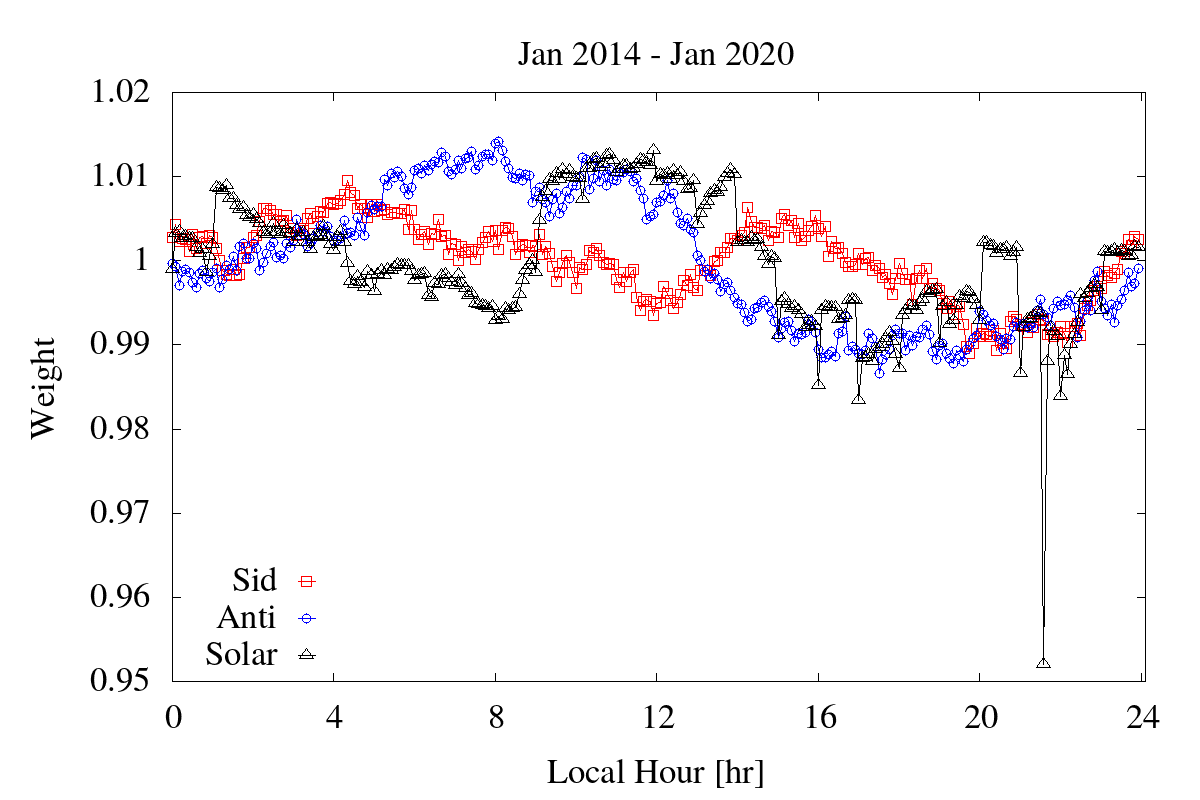
\includegraphics[width=0.5\textwidth]{weigth2014-2020_jan.png} 	
	\caption{Pesos de los hexágonos}
	\label{fig:wei_14_20}
\end{figure}

\section{Anisotropía}
El archivo de de todos los disparon empieza el Mon, 1 July 2013 12:05:08 GMT \footnote{$1372680308$}. Para trabajar en una cantidad entera de años, se trabaja a partir del  Thur, 1 January 2014 12:00:00 GMT \footnote{$1388577600$} y hasta el Thursday, 1 January 2020 12:00:00 GMT \footnote{$1577880000$}.  En este rango se tiene la tasa de eventos por día que se muestra en la Fig.\,\ref{tasa_total_diaria}.

\begin{figure}[H]
	\centering
	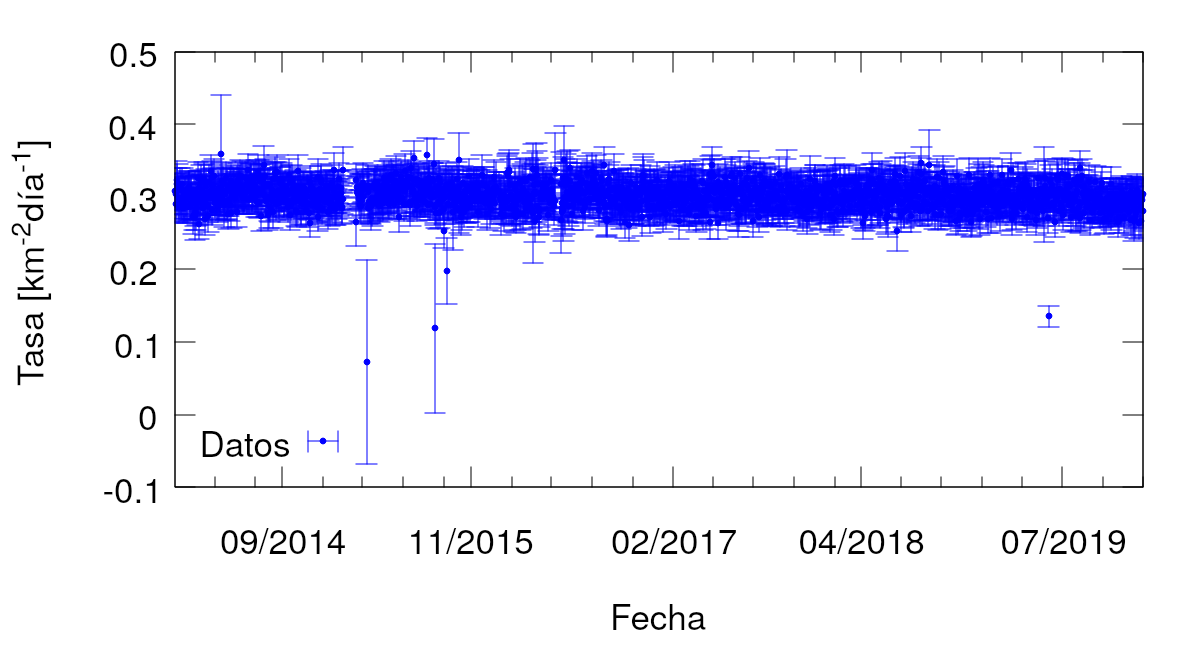
\includegraphics[width=0.5\textwidth]{rate_total.png}
	\caption{Tasa  de eventos en el rango de tiempo a trabajar}
	\label{tasa_total_diaria}
\end{figure}

\subsection{Lista detallada de los filtros aplicados de datos del herald}

\subsubsection{Datos para el análisis de anisotropía}
Esta sección muestra los filtros para los datos del análisis de anisotropía en el rango 1 EeV - 2 EeV.

\begin{enumerate}
	\item Energía entre  [1 EeV , 2 EeV)
	\item Rango de tiempo:
	\begin{itemize}
		\item[-] Inicial:1388577600 \\ (Thursday, 1 January 2014 12:00:00 GMT)
		\item[-] Final: 1577880000  \\ (Thursday, 1 January 2020 12:00:00 GMT)
	\end{itemize}
	\item Sectancia:  $\theta < 60^o$
	\item 6T5
	\item $ib=1$ Bad period flag. Un valor de 1 indica un buen periodo
\end{enumerate}

Con estos filtros se tienen $1\,092\,753$ eventos

\subsubsection{Datos para el cálculo de las correcciones del clima}

Estos son los filtros para los datos a utilizar para el cálculo de los parámetros del clima:

\begin{enumerate}
	\item Eventos con valor de señal de $S_{38}$\footnote{Valor de S38 sin la correccón del clima del paper del 2017} por encima de  $5.36\,\text{VEM}$. Este valor corresponde a $\sim 1\,$ EeV  en VEM.
	\item Rango de tiempo:
	\begin{itemize}
		\item[-] Inicial:1388577600 \\ (Thursday, 1 January 2014 12:00:00 GMT)
		\item[-] Final: 1577880000  \\ (Thursday, 1 January 2020 12:00:00 GMT)
	\end{itemize}
	\item Sectancia:  $\theta < 60^o$
	\item $iw<4$ (weather quality flag)
	\item 6T5
	\item $ib=1$ Bad period flag del herald.  Un valor de 1 indica un buen periodo
	\item $ib=1$ Bad period flag de los datos del clima. Un valor de 1 indica un buen periodo
\end{enumerate}


Con estos filtros se tienen $1\,208\,615$ eventos, con una tasa de eventos que se muestra en la Fig.\,\ref{tasa_total_diaria_ajuste_weather}. En la figura se observa que utilizando el corte en la señal de S38 sin corregir por la modulación del clima del herald \footnote{Las correcciones se calcularon para el archivo del disparo estándar} se observa una modulación anual.

\begin{figure}[H]
	\centering
	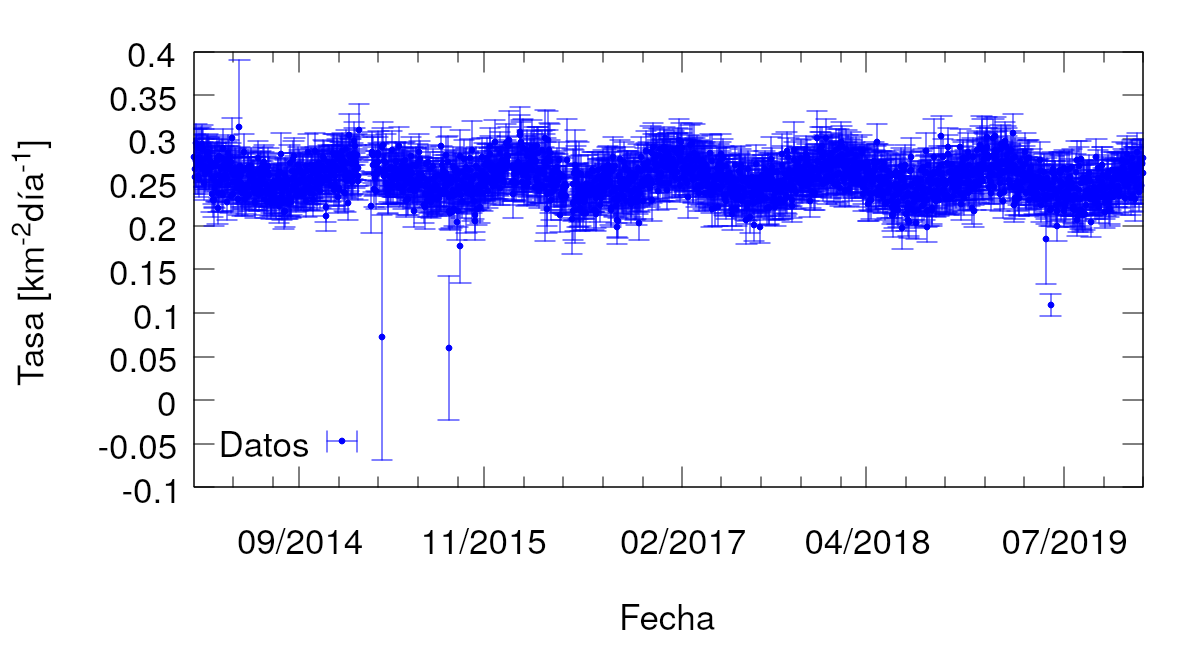
\includegraphics[width=0.5\textwidth]{rate_total_ajuste_weather.png}
	\caption{Tasa  de eventos en el rango de tiempo a trabajar para el ajuste de los parámetros del clima.}
	\label{tasa_total_diaria_ajuste_weather}
\end{figure}


\subsection{Análisis en frecuencia}

\begin{figure}[H]
	\centering
	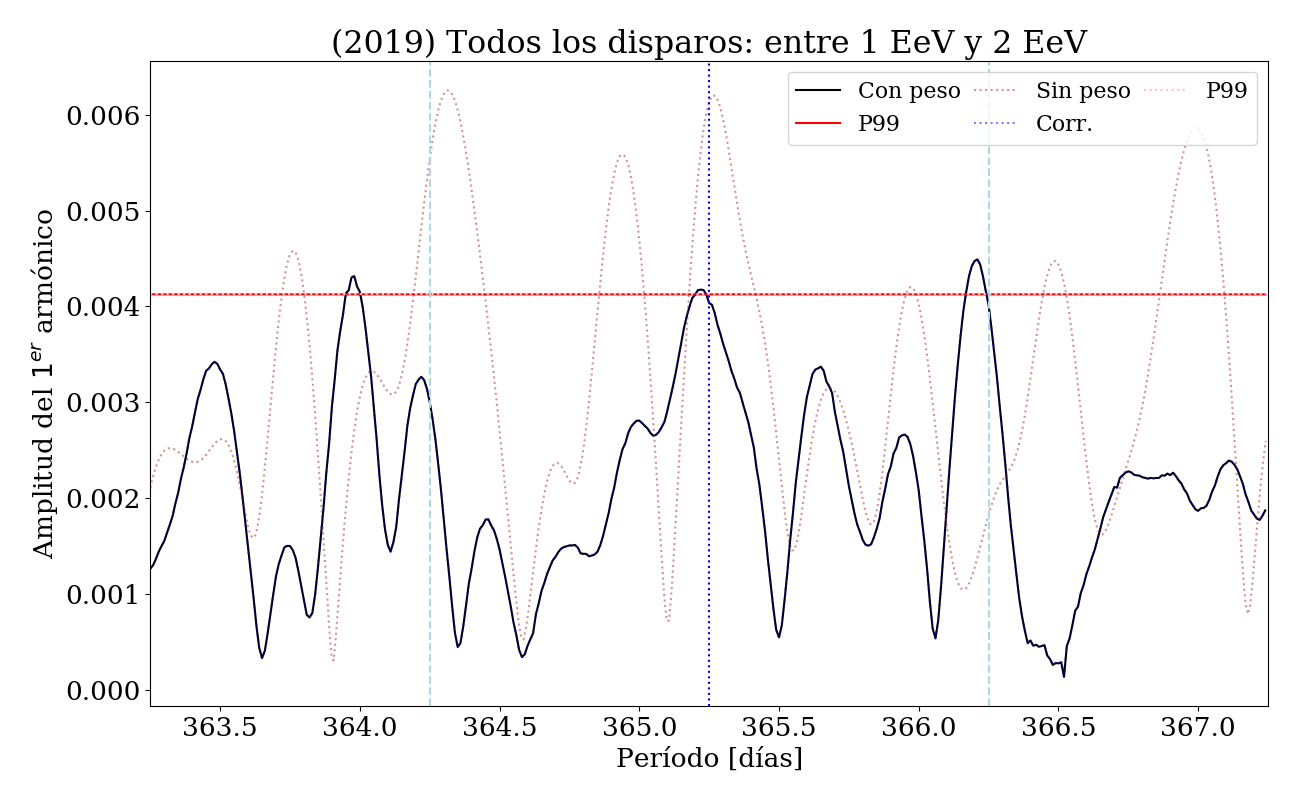
\includegraphics[width=0.5\textwidth]{2019_AllTriggers_1_2_EeV_con_vs_sin_peso.png}
	\caption{Análisis en frecuencia en ascensión recta en rango 1 EeV - 2 EeV}
	\label{fig:consin}
\end{figure}


\section{Corrección del clima}

\begin{figure}[H]
	\centering
	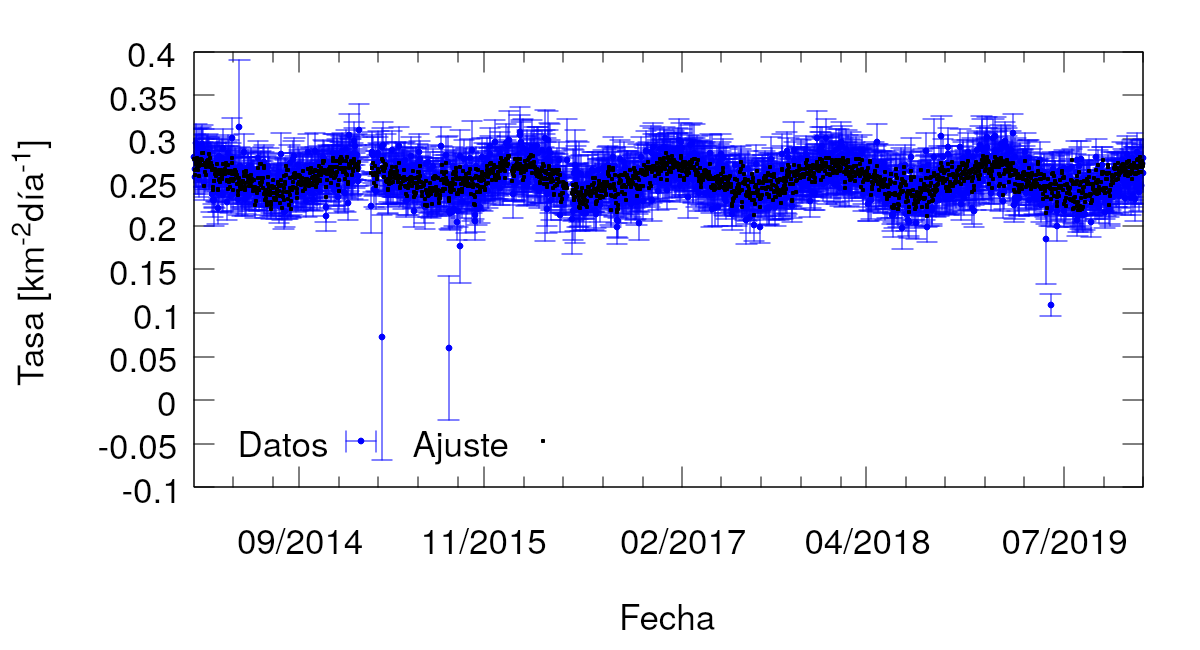
\includegraphics[width=0.5\textwidth]{rate_Ajuste.png}
\end{figure}


Aca estaba el mismo ajuste que más abajo!

La selección de los eventos genera dos conjuntos de datos: uno para el análisis de anisotropía en el bin 1 EeV - 2 EeV, y el segundo de los eventos con energía mayor a 1 Eev para obtener los parámetros del clima. En esta selección se tiene en cuentan los eventos de $\theta < 60^o$ , como también  los mismos que no se encuentren en un periodo de mala adquisición datos, este parámetro se denomina $ib$ de los \textbf{eventos del herald}. Este periodo consiste en momento donde el obsevatorio no recibe datos de las estaciones de clima o de los hexágonos. 

El parámetro de $ib$ de los \textbf{datos del clima} es irrelevante durante el proceso de filtrar eventos. Entra en juego cuando hago el análisis del clima, donde desecho los eventos que fueron recabados durante \emph{bad weather} \textbf{y} no fueron filtrados ya antes. 


\section{Pesos de los hexágonos}

Para constatar que no exista ninguna anomalía en los pesos de los hexágonos, se realiza el cálculo de los mismos para tres frecuencias de referencia para el análisis de anisotropías.  Los pesos se muestran en la Fig.\,\ref{fig:wei_14_20}. El rango de tiempo en el que se calculan estas curvas es entre 1 de Enero del 2014 y el 1 de Enero del 2020.

\begin{figure}[H]
	\centering
	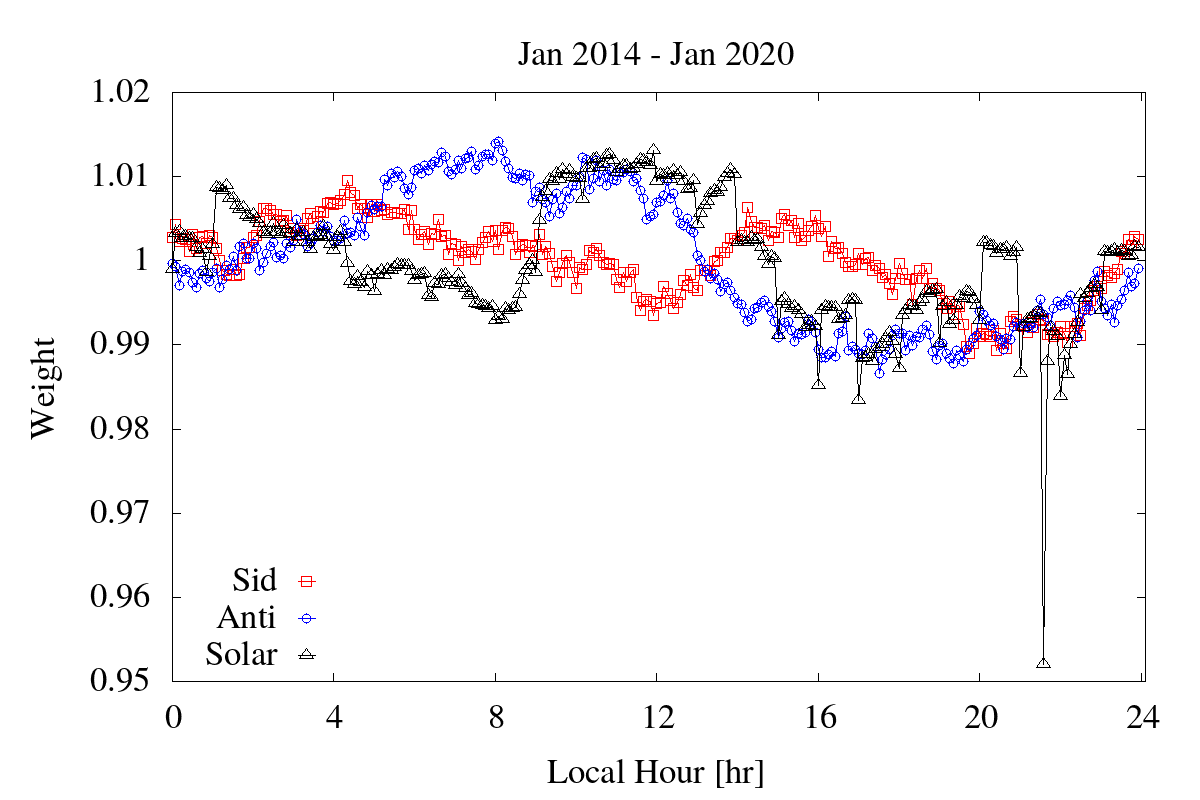
\includegraphics[width=0.5\textwidth]{weigth2014-2020_jan.png} 	
	\caption{Pesos de los hexágonos}
	\label{fig:wei_14_20}
\end{figure}

\section{Anisotropía}
El archivo de de todos los disparon empieza el Mon, 1 July 2013 12:05:08 GMT \footnote{$1372680308$}. Para trabajar en una cantidad entera de años, se trabaja a partir del  Thur, 1 January 2014 12:00:00 GMT \footnote{$1388577600$} y hasta el Thursday, 1 January 2020 12:00:00 GMT \footnote{$1577880000$}.  En este rango se tiene la tasa de eventos por día que se muestra en la Fig.\,\ref{tasa_total_diaria}.

% En el rango $1372680308$ \footnote{Mon, 1 July 2013 12:05:08 GMT} y $1388577600$ \footnote{Thur, 1 January 2014 12:00:00 GMT}, la tasa de eventos del archivo $\text{All Triggers}$, tenía una tasa de eventos por debajo de lo normal. Por esto, se utiliza los eventos a partir del  1388577600. La tasa de eventos que se utiliza se puede ver a continuación:

\begin{figure}[H]
	\centering
	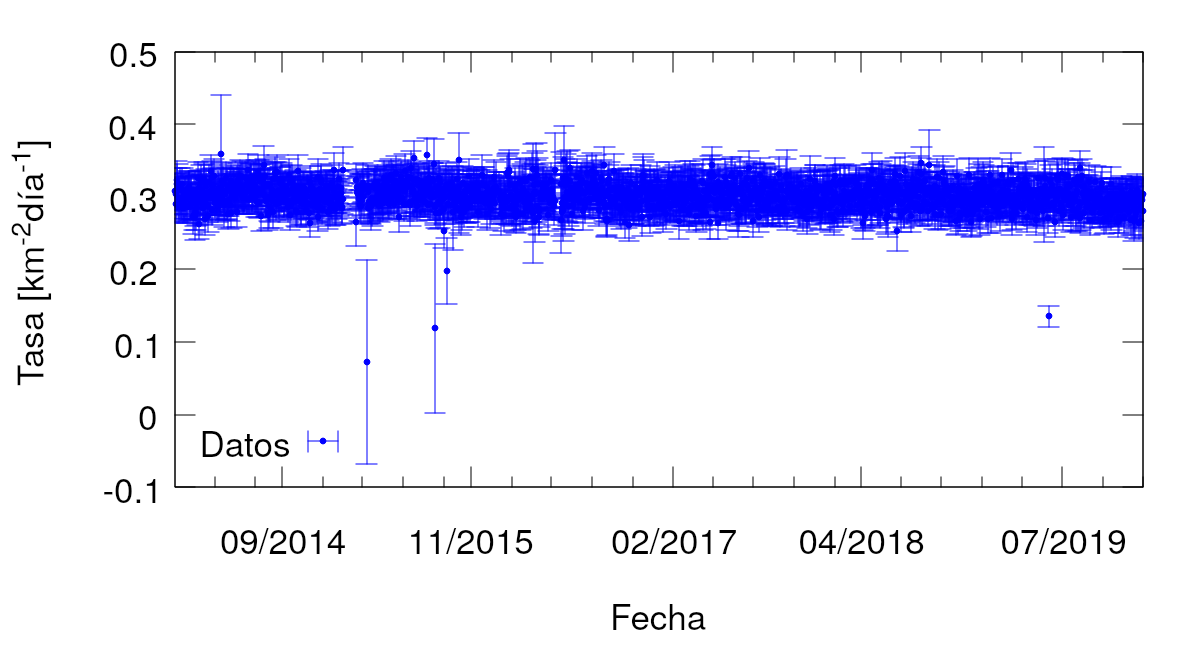
\includegraphics[width=0.5\textwidth]{rate_total.png}
	\caption{Tasa  de eventos en el rango de tiempo a trabajar}
	\label{tasa_total_diaria}
\end{figure}

\subsection{Lista detallada de los filtros aplicados de datos del herald}

\subsubsection{Datos para el análisis de anisotropía}
Esta sección muestra los filtros para los datos del análisis de anisotropía en el rango 1 EeV - 2 EeV.

\begin{enumerate}
	\item Energía entre  [1 EeV , 2 EeV)
	\item Rango de tiempo:
	\begin{itemize}
		\item[-] Inicial:1388577600 \\ (Thursday, 1 January 2014 12:00:00 GMT)
		\item[-] Final: 1577880000  \\ (Thursday, 1 January 2020 12:00:00 GMT)
	\end{itemize}
	\item Sectancia:  $\theta < 60^o$
	\item 6T5
	\item $ib=1$ Bad period flag. Un valor de 1 indica un buen periodo
\end{enumerate}

Con estos filtros se tienen $1\,092\,753$ eventos

\subsubsection{Datos para el cálculo de las correcciones del clima}

Estos son los filtros para los datos a utilizar para el cálculo de los parámetros del clima:

\begin{enumerate}
	\item Eventos con valor de señal de $S_{38}$\footnote{Valor de S38 sin la correccón del clima del paper del 2017} por encima de  $5.36\,\text{VEM}$. Este valor corresponde a $\sim 1\,$ EeV  en VEM.
	\item Rango de tiempo:
	\begin{itemize}
		\item[-] Inicial:1388577600 \\ (Thursday, 1 January 2014 12:00:00 GMT)
		\item[-] Final: 1577880000  \\ (Thursday, 1 January 2020 12:00:00 GMT)
	\end{itemize}
	\item Sectancia:  $\theta < 60^o$
	\item $iw<4$ (weather quality flag)
	\item 6T5
	\item $ib=1$ Bad period flag del herald.  Un valor de 1 indica un buen periodo
	\item $ib=1$ Bad period flag de los datos del clima. Un valor de 1 indica un buen periodo
\end{enumerate}


Con estos filtros se tienen $1\,208\,615$ eventos, con una tasa de eventos que se muestra en la Fig.\,\ref{tasa_total_diaria_ajuste_weather}. En la figura se observa que utilizando el corte en la señal de S38 sin corregir por la modulación del clima del herald \footnote{Las correcciones se calcularon para el archivo del disparo estándar} se observa una modulación anual.

\begin{figure}[H]
	\centering
	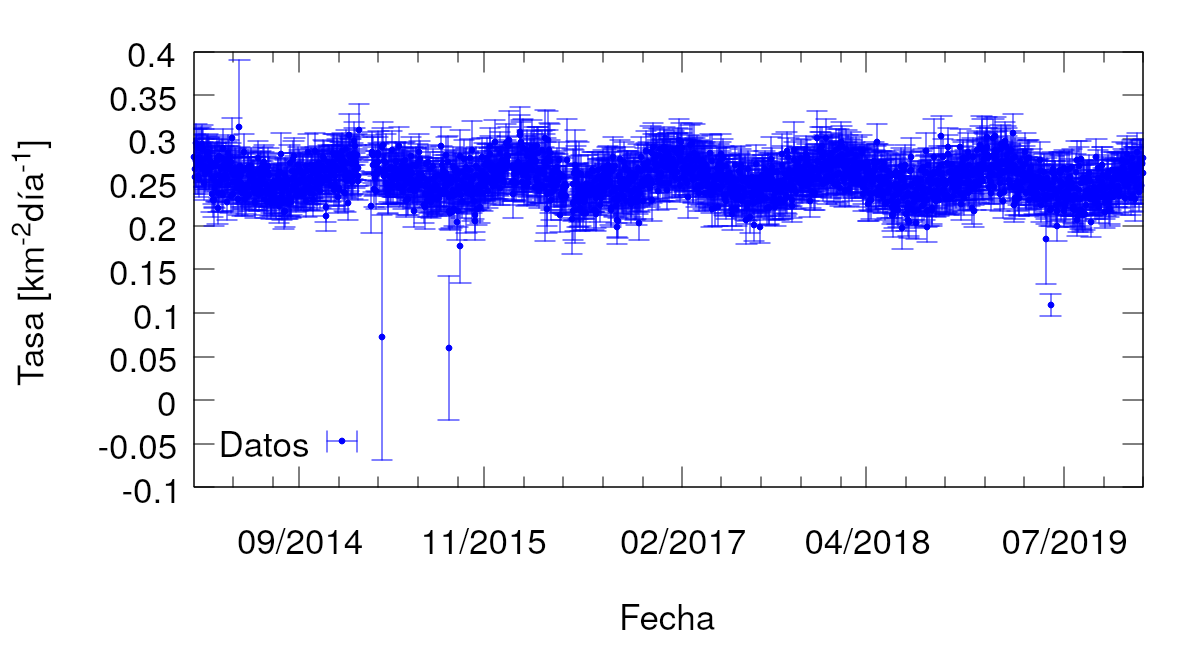
\includegraphics[width=0.5\textwidth]{rate_total_ajuste_weather.png}
	\caption{Tasa  de eventos en el rango de tiempo a trabajar para el ajuste de los parámetros del clima.}
	\label{tasa_total_diaria_ajuste_weather}
\end{figure}


\subsection{Análisis en frecuencia}

\begin{figure}[H]
	\centering
	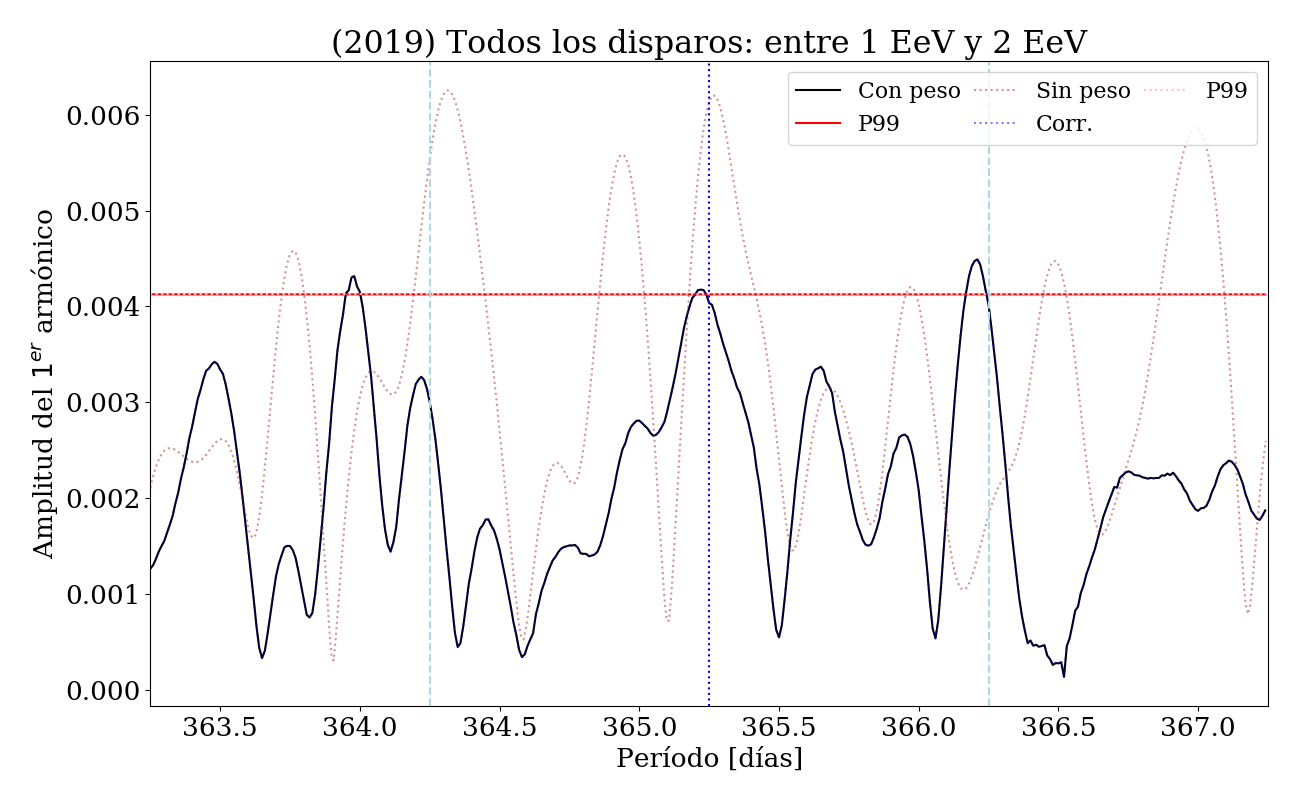
\includegraphics[width=0.5\textwidth]{2019_AllTriggers_1_2_EeV_con_vs_sin_peso.png}
	\caption{Análisis en frecuencia en ascensión recta en rango 1 EeV - 2 EeV}
	\label{fig:consin}
\end{figure}


\section{Corrección del clima}

\begin{figure}[H]
	\centering
	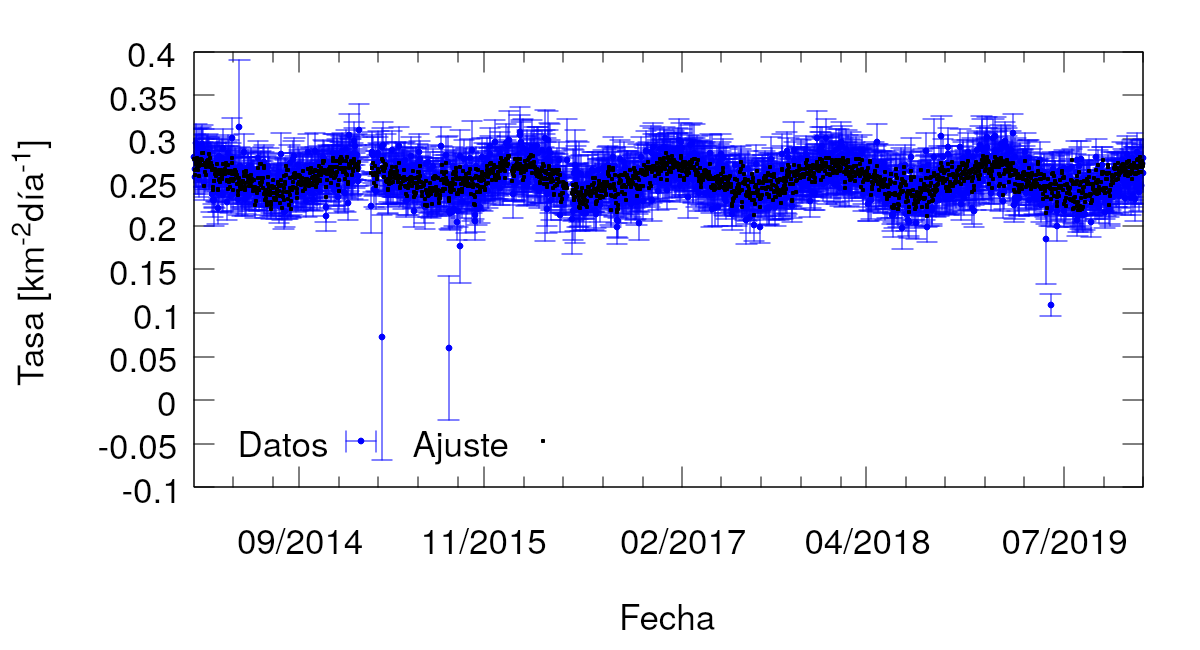
\includegraphics[width=0.5\textwidth]{rate_Ajuste.png}
\end{figure}

%%%%%%%%5
\begin{figure}[H]
\begin{subfigure}{.5\textwidth}
	\centering
	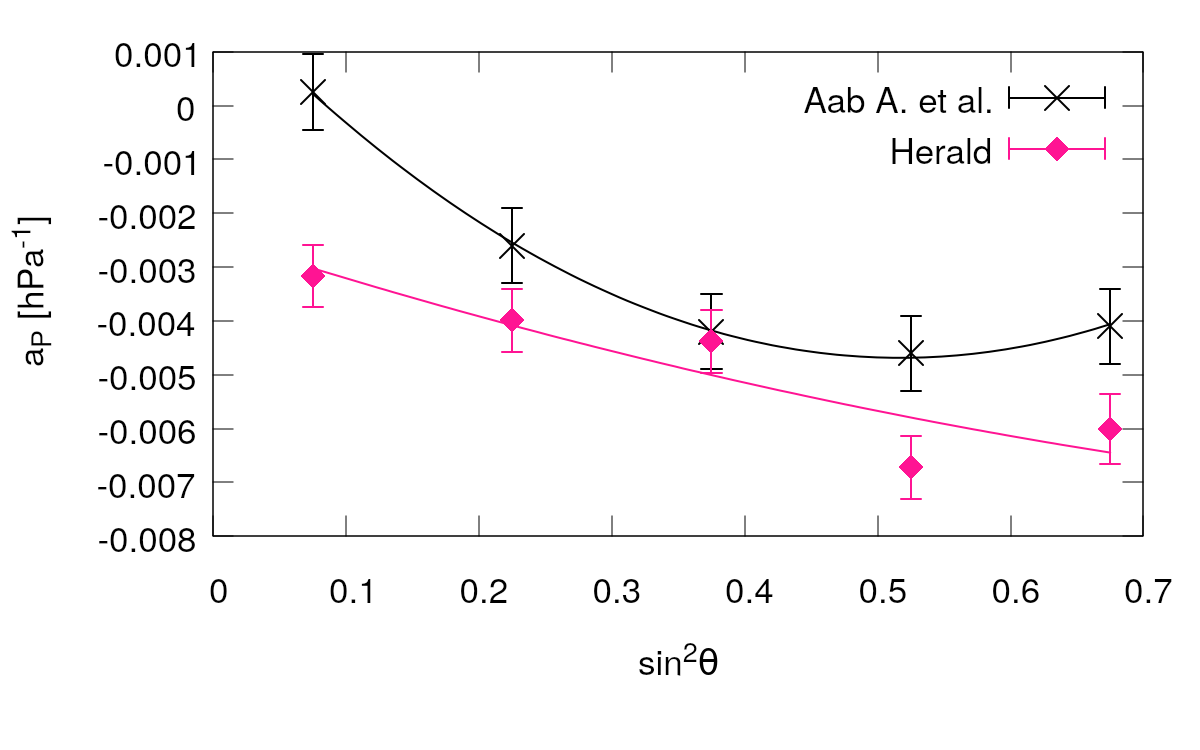
\includegraphics[width=\linewidth]{ap_6t5.png}
	\caption{Parámetro de clima $a_P$}
\end{subfigure}%
\begin{subfigure}{.5\textwidth}
	\centering
	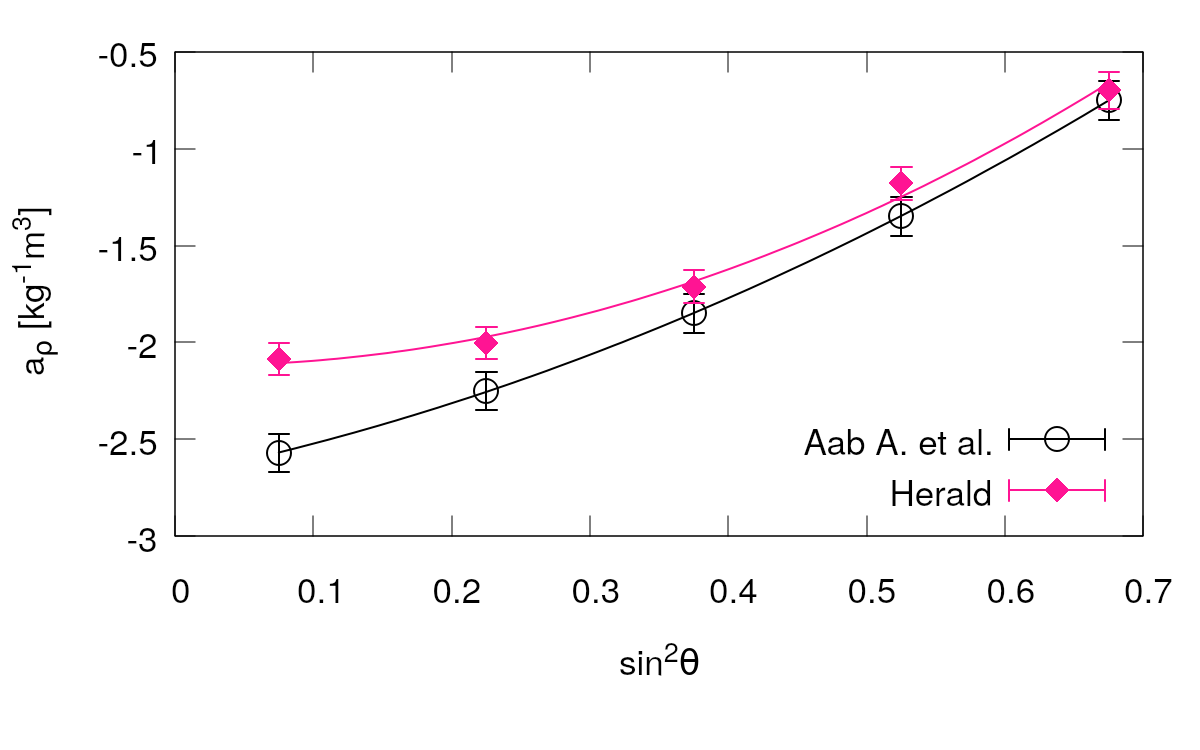
\includegraphics[width=\linewidth]{arho_6t5.png}
	\caption{Parámetro de clima $a_\rho$}
\end{subfigure}\\
\centering
\begin{subfigure}{.5\textwidth}
	\centering
	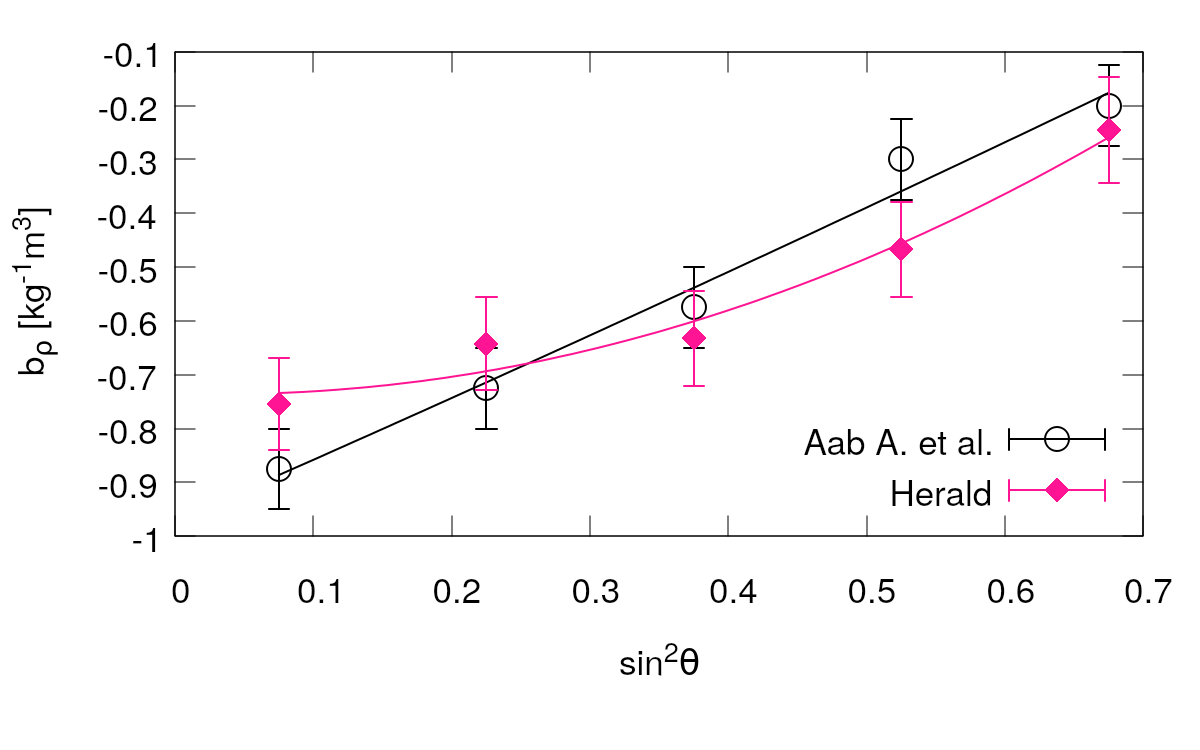
\includegraphics[width=\linewidth]{brho_6t5.png}
	\caption{Parámetro de clima $b_\rho$}
\end{subfigure}%
\caption{Parámetros de clima calculados para la corrección del archivo de todos los disparos}
\end{figure}
%%%%%%%%


%%%%%%%%%%%%%%%%%%%%%%%%%%%%%%%%%%%%%%%%%%%%%%%%%%%%%%%%%%%%%%%%%%%%%%%%%%%%%%%%%%%%%%%%%
%%%%%%%%%%%%%%%%%%%%%%%%%%%%%%%%%%%%%%%%%%%%%%%%%%%%%%%%%%%%%%%%%%%%%%%%%%%%%%%%%%%%%%%%%
%%%%%%%%%%%%%%%%%%%%%%%%%%%%%%%%%%%%%%%%%%%%%%%%%%%%%%%%%%%%%%%%%%%%%%%%%%%%%%%%%%%%%%%%%

      \subsubsection{Modulación del clima para todos los triggers}

      Para corroborar los parámetros del clima, primero calculé las tasas de eventos de los archivos del 2017 y 2020 para energías mayores a 1  EeV, donde obtuve los siguientes gráficos Fig.\ref{fig:rate_daily_2017_1EeV} y \ref{fig:rate_daily_2020_1EeV}. 

        \begin{figure}[H]
        
          \begin{subfigure}[b]{0.5\textwidth}
          \centering
          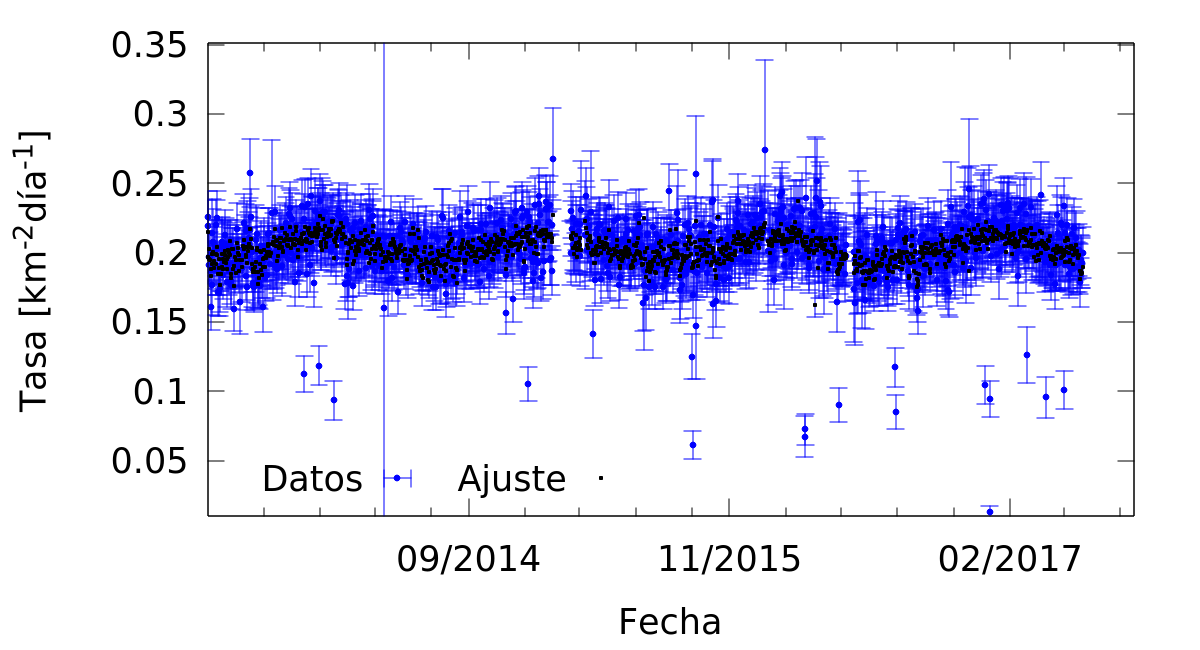
\includegraphics[width=\textwidth]{../0_Introduccion/daily_rate/daily_rate_AllTriggers_2017_1EeV.png}
          \caption{Archivo de 2017}   \label{fig:rate_daily_2017_1EeV}
          \end{subfigure}%
        \hfill
          \begin{subfigure}[b]{0.5\textwidth}
          \centering
          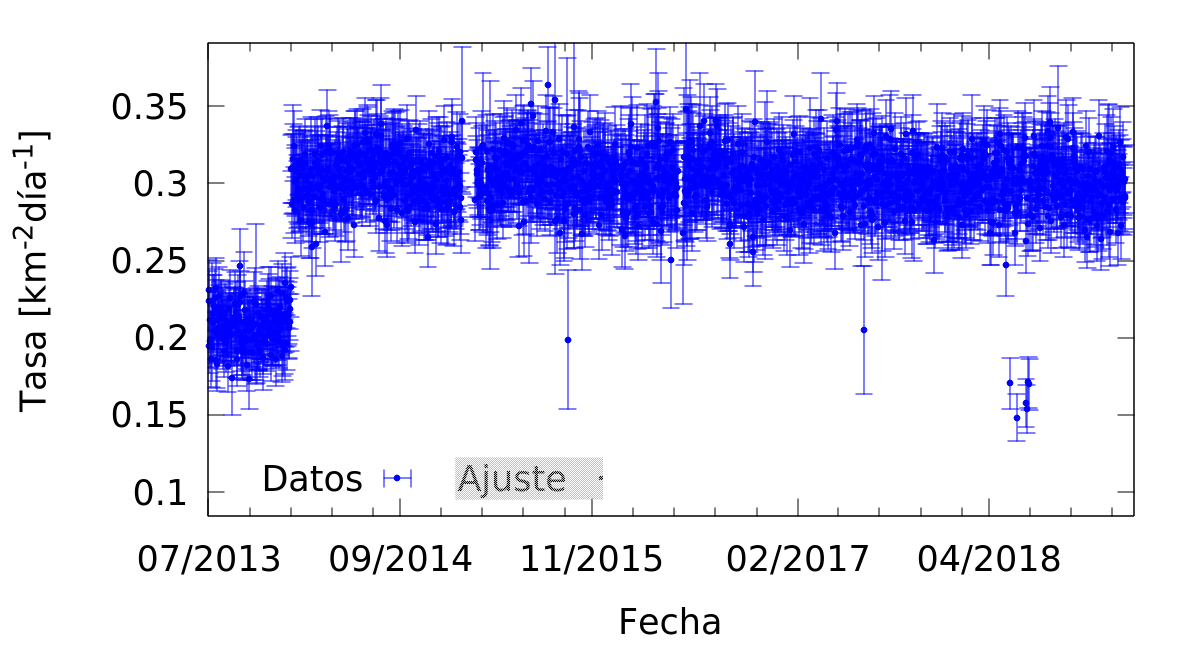
\includegraphics[width=\textwidth]{../0_Introduccion/daily_rate/daily_rate_AllTriggers_2019_1EeV.png}
          \caption{Archivo del 2020}  \label{fig:rate_daily_2020_1EeV}
          \end{subfigure}
          \caption{Tasa de eventos diaria por encima de 1 EeV para los datos de todos los disparos.}
        \end{figure}

      Después calculé los parámetros del clima para energía mayores a 1 EeV. Para el archivo de 2017 obtuve la Fig.\,\ref{fig:parameters_2017_1EeV}. Los comparé con el paper del weather del main array, para ver si dan algo razonable. Verifiqué las siguientes cosas para el ajuste

      \begin{itemize}
        \item Me fijé que delay en la densidad cada momento fuera de dos  horas
        \item Me fijé que el ajuste no tuviera en cuenta periodos malos, bad periods
        \item Me fijé que el delay de la densidad media también fuera tal que para cada evento estuviera centrada $\pm$12 horas
        \item También me fijé que el rango de tiempo estuviera bien, porque estos datos están disponibles desde el 2013  recién
        \item Me fijé que los $\chi^2$ reducido fuera algo razonable. Todos rondaban alrededor de $1.05$
      \end{itemize}

      EL rango de tiempo que usé fue este: 
      \begin{itemize}
        \item Inicio: 1372680308
        \item Final: 1496275090
      \end{itemize}
        \begin{figure}[H]
          \begin{subfigure}[b]{0.5\textwidth}
          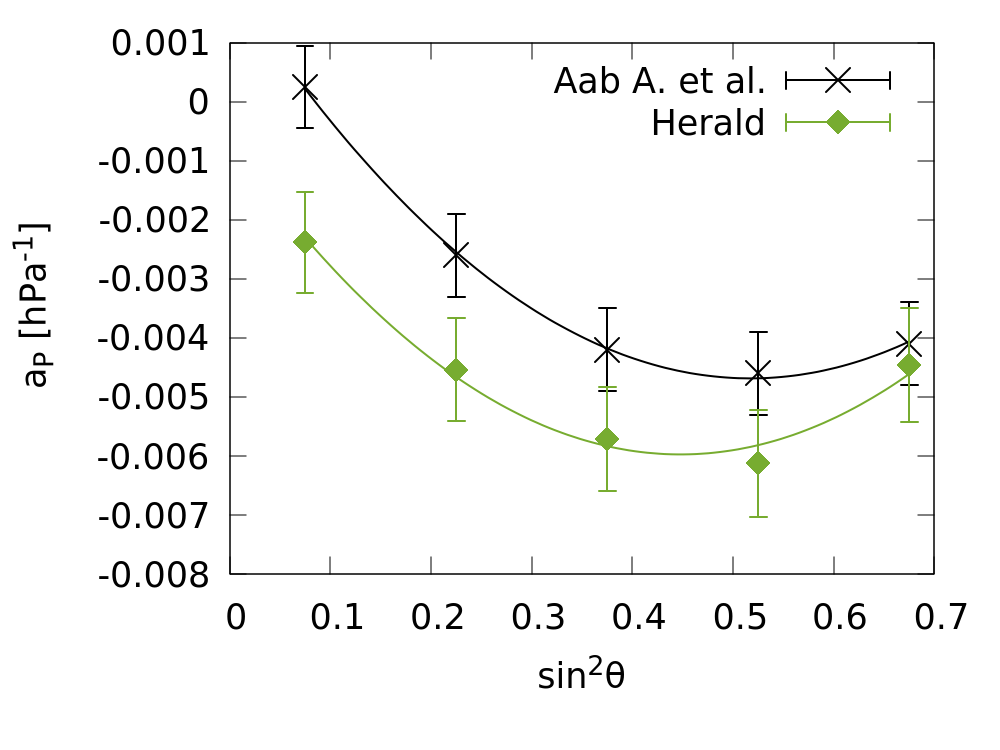
\includegraphics[width=\linewidth]{../0_Introduccion/params/ap_2017_above_1EeV.png}
          \caption{Parámetro $a_P$ }
          \label{fig:ap_2017_1EeV}
          \end{subfigure}%
          \hspace{\fill}
          \begin{subfigure}[b]{0.5\textwidth}
          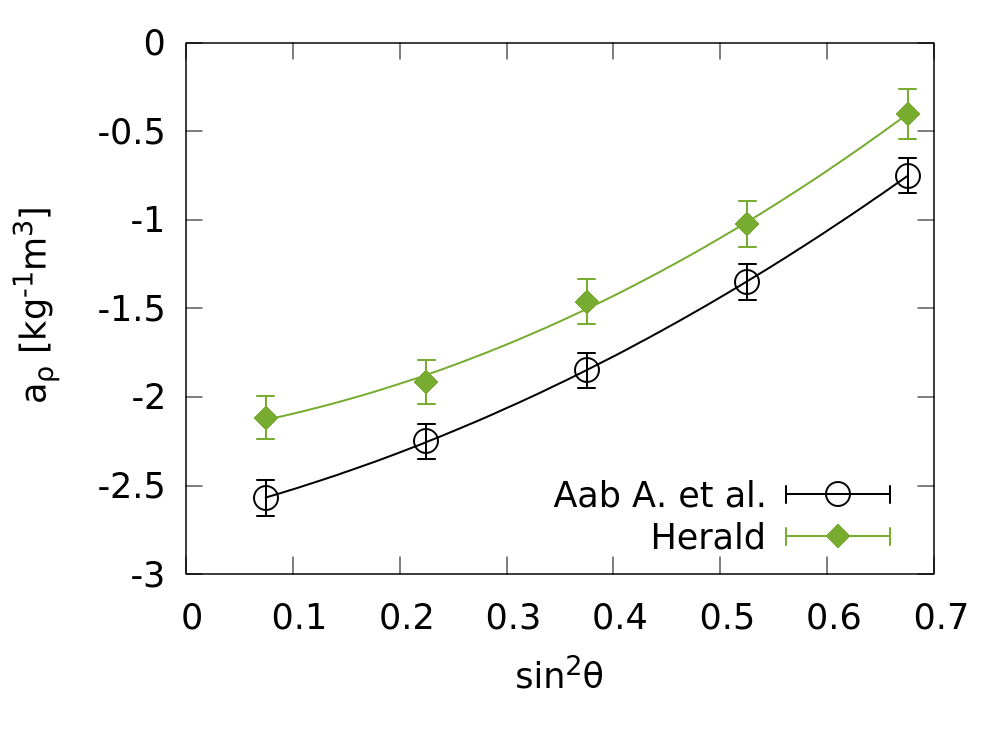
\includegraphics[width=\linewidth]{../0_Introduccion/params/arho_2017_above_1EeV.png}
          \caption{Parámetro $a_{\rho}$ }
          \label{fig:arho_2017_1EeV}
          \end{subfigure}%
          \hspace{\fill}
          \begin{subfigure}[b]{\textwidth}
          \centering
          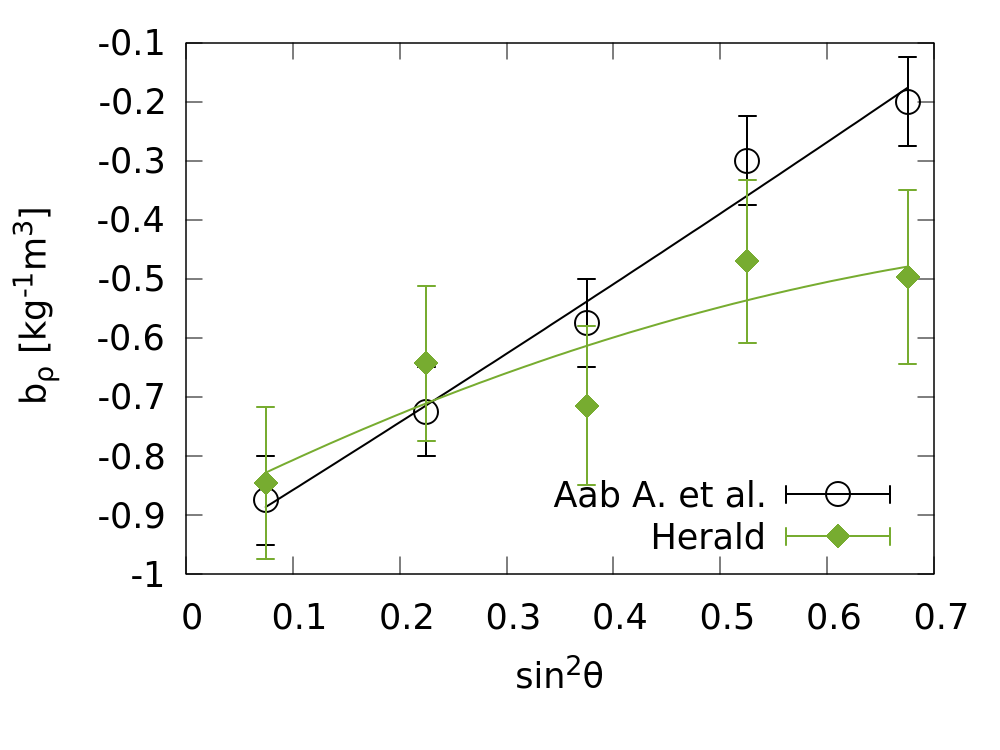
\includegraphics[width=0.5\linewidth]{../0_Introduccion/params/brho_2017_above_1EeV.png}
          \caption{Parámetro  $b_\rho$   }
          \label{fig:brho_2017_1EeV}
          \end{subfigure}%
          \caption{Parámetros de la modulación del clima considerando los datos para todos los disparos de 2017. Los mismos se comparan con los ajustes obtenidos en \cite{aab2017impact}.}\label{fig:parameters_2017_1EeV}
        \end{figure}

        Lo que más me llama la atención es el comportamiento del parámetro $b_\rho$, que como se discutió en otras oportunidades, tiene que ver con el parámetro $a_\rho$ con una razón de  $1:3$ más o menos. 



      Hacemos el mismo procedimiento con el archivo 2020, {\bf pero filtrando los eventos por el valor de S38 sin corregir por la modulación del clima}. Para calcular la tasa y los parámetros del clima, se toman los eventos después de ese salto de 0.2 a 0.3, obtengo los siguientes resultados:

        \begin{figure}[H]
          \centering
          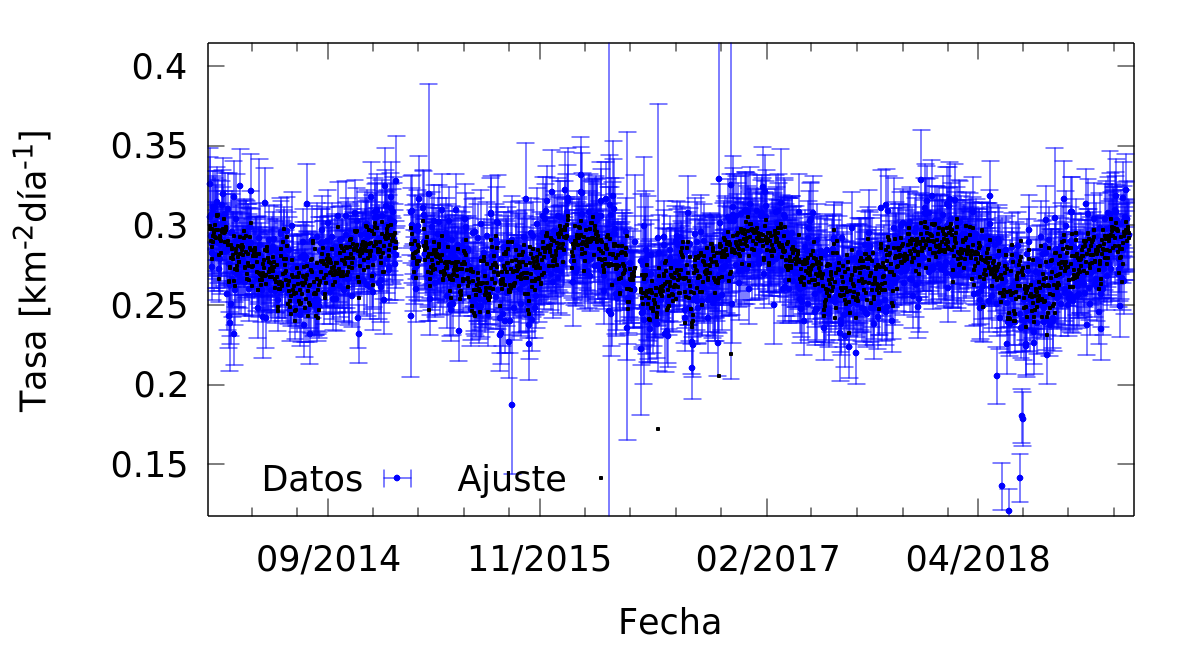
\includegraphics[width=0.5\textwidth]{../0_Introduccion/daily_rate/daily_rate_AllTriggers_2020_1EeV.png}
        \end{figure}

      Acá también verifiqué lo mismo que el caso anterior, lo único que ahora el $\chi^2$ rondaba alrededor de los $1.08$. Siempre verifico que no sea mucho mayor o menor a 1.

      EL rango de tiempo que usé para este caso fue este: 
      \begin{itemize}
        \item Inicio: 1388910508
        \item Final: 1550490858
      \end{itemize}
      
        \begin{figure}[H]
          \begin{subfigure}[b]{0.5\textwidth}
          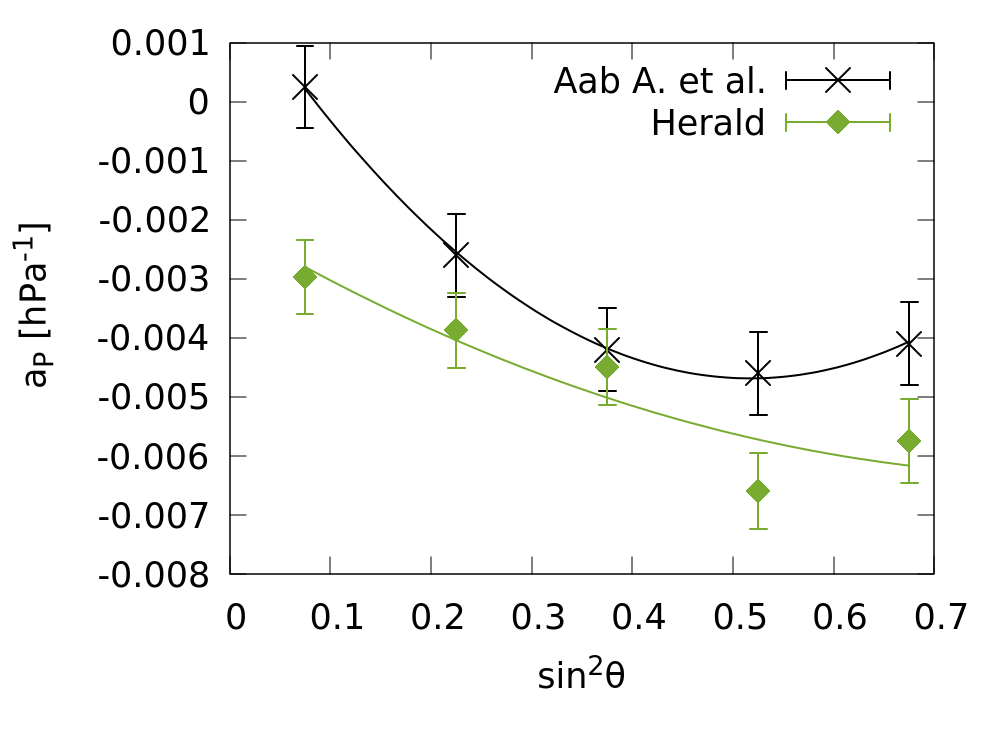
\includegraphics[width=\linewidth]{../0_Introduccion/params/ap_2020_above_1EeV.png}
          \caption{Parámetro $a_P$ }
          \label{fig:ap_2020_1EeV}
          \end{subfigure}%
          \hspace{\fill}
          \begin{subfigure}[b]{0.5\textwidth}
          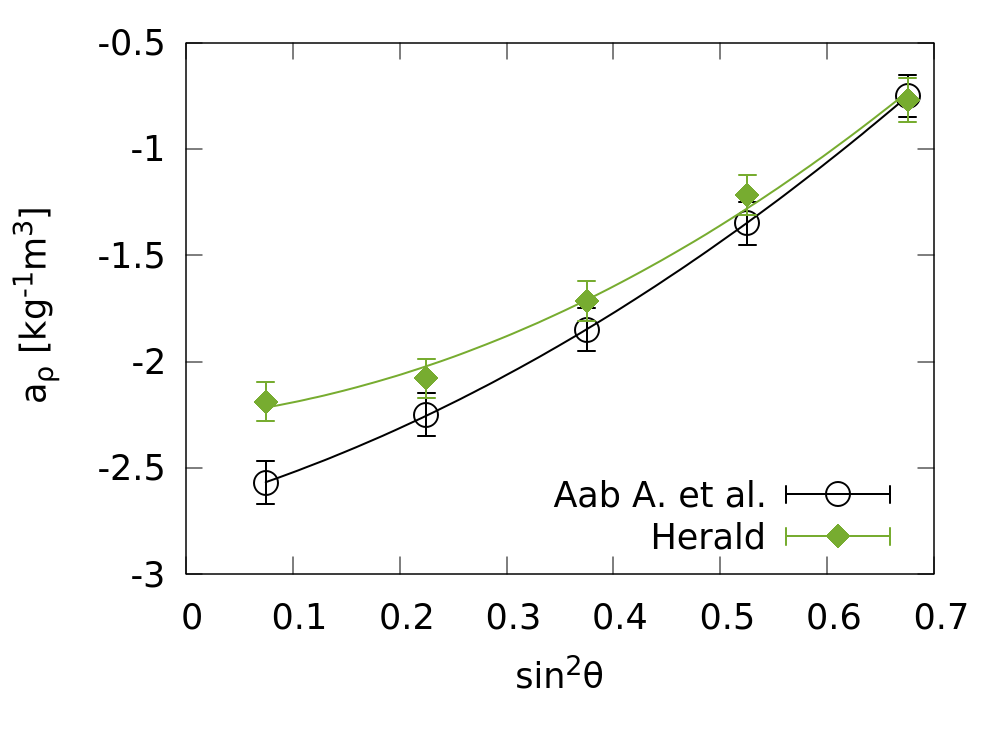
\includegraphics[width=\linewidth]{../0_Introduccion/params/arho_2020_above_1EeV.png}
          \caption{Parámetro $a_{\rho}$ }
          \label{fig:arho_2020_1EeV}
          \end{subfigure}%
          \hspace{\fill}
          \begin{subfigure}[b]{\textwidth}
          \centering
          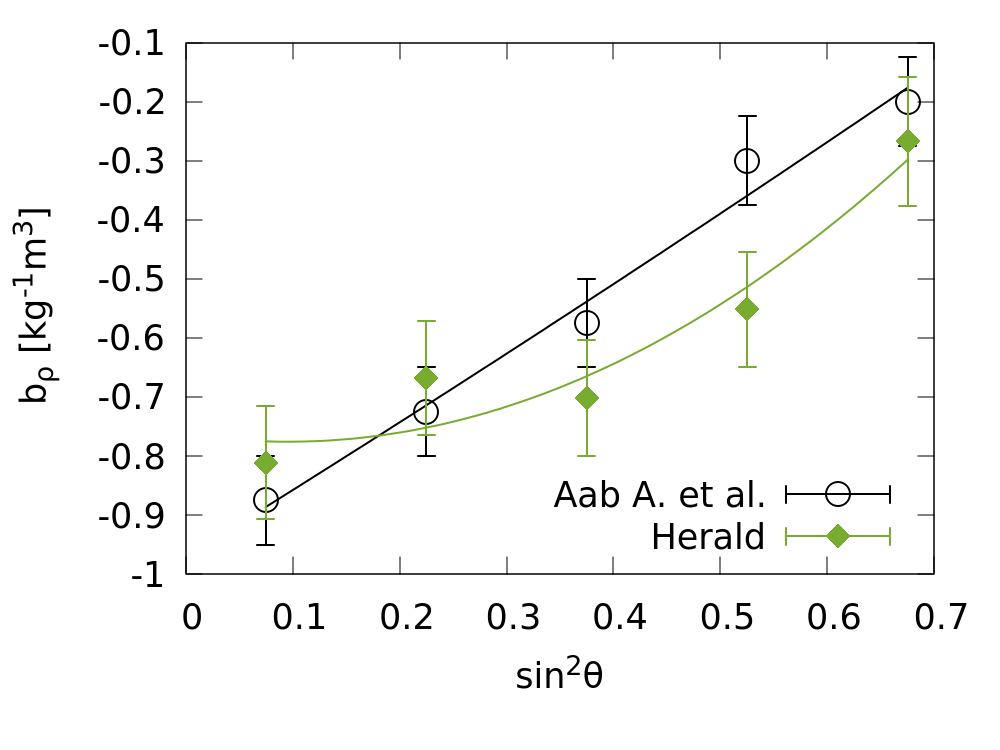
\includegraphics[width=0.5\linewidth]{../0_Introduccion/params/brho_2020_above_1EeV.png}
          \caption{Parámetro  $b_\rho$   }
          \label{fig:brho_2020_1EeV}
          \end{subfigure}%
          \caption{Parámetros de la modulación del clima considerando los datos para todos los disparos de 2020. Los mismos se comparan con los ajustes obtenidos en \cite{aab2017impact}.}\label{fig:parameters_2020_1EeV}
        \end{figure}



      Considerando el filtro con el S38 en el archivo 2020 y la energía en el 2017, quiero saber si obtengo parametros  del clima comparables. Ya que el Main Array se corresponden los parametros del 2015 y 2019, yo esperaría que con todos los triggers pase los mismo. Una diferencia importante entre ambos análisis es que los parametros del 2020 contienen eventos hasta el 31/12/2019.


        \begin{figure}[H]
          \begin{subfigure}[b]{0.5\textwidth}
          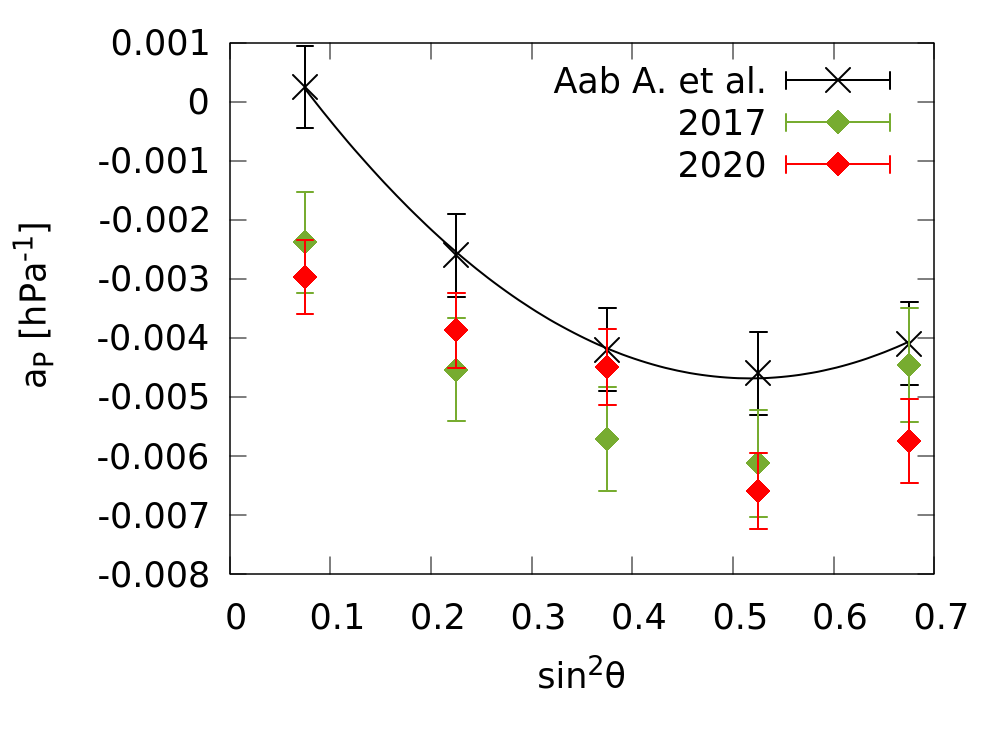
\includegraphics[width=\linewidth]{../0_Introduccion/params/ap_2017_2020_above_1EeV.png}
          \caption{Parámetro $a_P$ }
          \end{subfigure}%
          \hspace{\fill}
          \begin{subfigure}[b]{0.5\textwidth}
          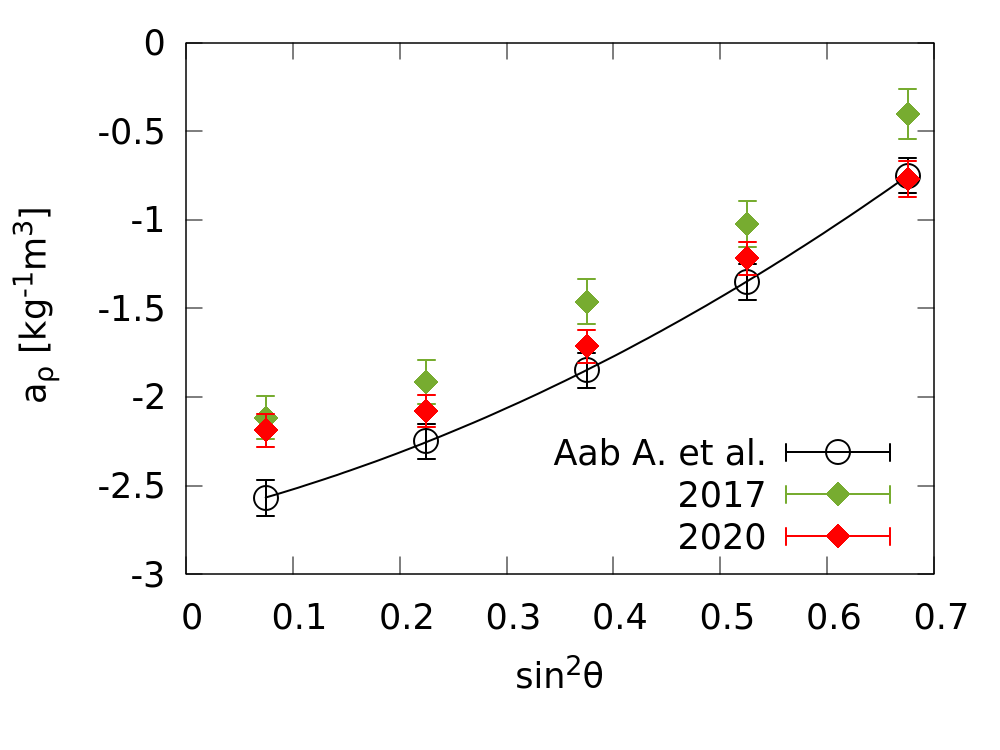
\includegraphics[width=\linewidth]{../0_Introduccion/params/arho_2017_2020_above_1EeV.png}
          \caption{Parámetro $a_{\rho}$ }
          \end{subfigure}%
          \hspace{\fill}
          \begin{subfigure}[b]{\textwidth}
          \centering
          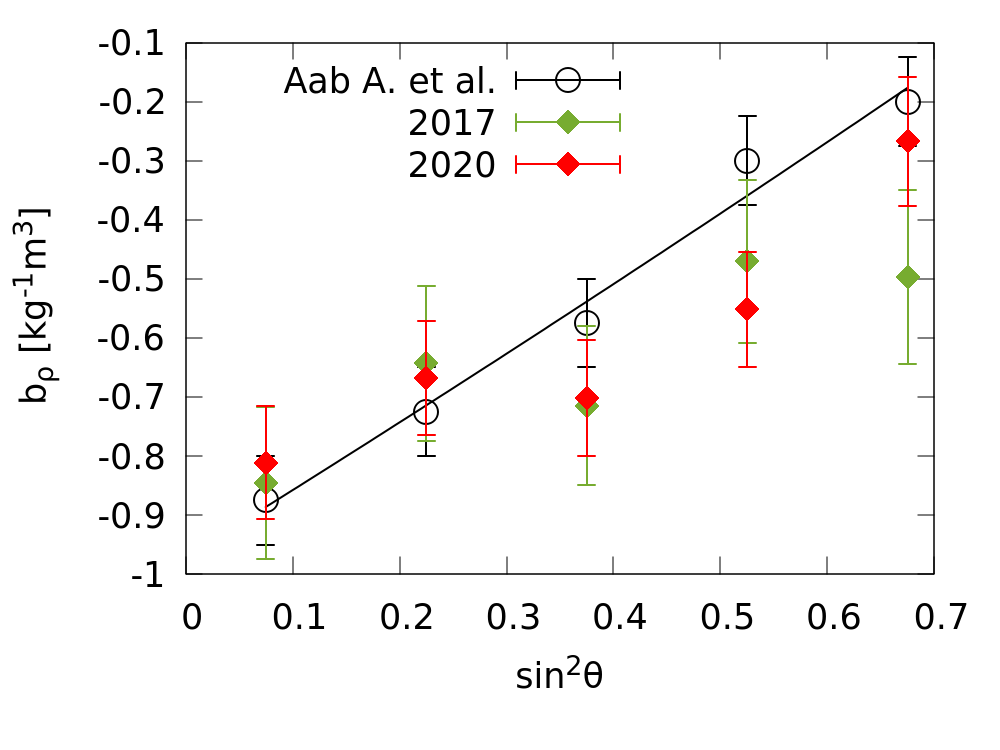
\includegraphics[width=0.5\linewidth]{../0_Introduccion/params/brho_2017_2020_above_1EeV.png}
          \caption{Parámetro  $b_\rho$   }
          \end{subfigure}%
          \caption{Parámetros de la modulación del clima considerando los datos para todos los disparos del archivo 2017 y 2020. Los mismos se comparan con los ajustes obtenidos en \cite{aab2017impact}.}
        \end{figure}

      Se ve que estos parametros no son comparables. 
